\chapter{Background}

% lets add lit review
% email has template  

\section{Agriculture \& Climate Change}

Climate change is a rising global issue with long term affects. One observed consequence includes the increase in temperature globally. From 1850 to 2018 the global temperature has increased by 1.41$^ \circ $C, which has caused an increase in warmer and more unpredictable weather \cite{agriculturalAdaptationAnderson}.

Due to the increase in temperature, the growing season in Scotland has lengthened, and therefore increased the yield in produce. Between 1960-2006 the main crop of Scotland, potatoes, have increased by 30-35 t/ha (tonnes per hectares). This can also be due to a more modern variety of potato that have greater resistance to diseases \cite{ScotlandGregory}. This increase in yield has not only fed the population, but has created more jobs and increased income into the country.

Rising temperatures can also lead to an increase in extreme weather conditions. As we can see in the Hindu-Kush Himalayan region, there has already been an increase of these occurrences in the last decade: with an increase in landslides, floods, droughts and pests, this has caused a drop in food production and income for the locals \cite{HinduKushHussain}. It can also lead to major health related issues for the locals.

To regulate and predict yields, farms all across the world have began to introduce machine learning methods into their production techniques. One farm growing coffee have implemented image processing algorithms to count the number of coffee fruits on a branch \cite{coffeeCountRamos}. The Machine Vision System then uses a linear estimation model to classify whether fruits can be categorised into either "harvestable, not harvestable, and fruits whose maturation stage were disregarded" \cite{coffeeCountRamos}. By classifying fruits into whether they can be harvestable or not creates a more accurate prediction for farmers when trying to meet demands by consumers.

Another use for machine learning in agriculture is that it can be used to identify pests and diseases. One article \cite{strawberryThrips} spoke of using SVM (Support Vector Machine), a type of supervised learning to detect thrips in strawberry greenhouses. The SVM model uses a number of parameters such as the diameters, hue, saturation and intensity of colour to classify whether strawberries in the greenhouse had thrips.

The advantage of having image processing models detect diseases and pests automatically, is that it saves man power and time, as farmers do not have to check by hand so see if there are problems with their produce. The other positive, is that this method saves money and soil as there is less use of chemical pesticides \cite{MLAgricultureLiakos}. These are expensive and can have significant negative impacts environmentally: residue can be left on crops and the chemicals can pollute water as well as affect local wildlife.

\subsection{Precision Agriculture}




\section{Machine Learning}

“Machine learning is a branch of artificial intelligence and computer science which focuses on the use of data and algorithms to imitate the way that humans learn, gradually improving its accuracy” \cite{machineLearningIBM}. Algorithms can do this by checking their output against the training data, calculating the deviation, and making adjustments as necessary.

Generally, a supervised machine learning model contains the following three components
\begin{enumerate}
    \item Decision process
    \item Error function
    \item Updating or optimising process
\end{enumerate}

The decision process consists of an input data (that can either be labelled or unlabelled) which the algorithm will use to estimate patterns and classifications. This is then followed by the error function which will evaluate the previous estimate. By comparing to known examples, the error function will make a comparison to see how accurate the estimate was.
Finally, the model optimisation process will use the evaluation from the error function to adjust weights, ideally reducing discrepancies between the estimate and the data. This entire process is then repeated to optimise the model until the threshold of accuracy is met \cite{machineLearningIBM} \cite{machineLearningBerkeley} \cite{machineLearningNvidia}.

\subsection{Types of Machine Learning}

There are a few different types of models for machine learning. Here we will go through a few of the more well-known types to understand what they are and how they can be integrated into agriculture to help with the food crisis.

\subsubsection{Reinforcement Learning}

Reinforcement learning is not trained using sample data. Instead it uses a reward/punishment system. As the AI agent explores through a problem space, the dataset offers rewards for accomplishing goals and punishments for not doing well. The agent relies on its previous experiences and explores the space for better rewards. This is an iterative process, and so the more iterations the agent has been through, the better the model will get. The end goal for the agent is the best cumulative reward and therefore the optimal method to accomplish a goal \cite{machineLearningIBM} \cite{machineLearningNvidia}.

In the field of agriculture, the rewards would not be immediately accessible as the reward would depend on the harvest, which is determined at the end of the growth season for each type of produce. As our dataset does not have a punishments and rewards system, this would be an inappropriate model to use.

\subsubsection{Unsupervised Learning}

Unsupervised learning takes an input of unlabelled data, and so does not necessarily have clear instructions on what to do with it. The algorithm tries to identify patterns and clustering within the data without the need for human interaction. The dataset is often unlabelled because labelled data can be hard or expensive to come by. Due to the fact the dataset is not labelled, it can be hard to measure the accuracy of unsupervised models \cite{machineLearningIBM} \cite{machineLearningNvidia}.

Unsupervised learning takes in an input of unlabelled data with no particular goal in mind other than clustering and identifying relationships in the data. As we are able to provide labelled data and have a specific goal in mind, this model is not suitable for precision agriculture.

\subsubsection{Supervised Learning}

A supervised learning model is the opposite of the unsupervised learning model in that the input dataset is labelled and classified. This type of machine learning is good for classification and regression problems. The advantage of having a labelled dataset is that the model can correct itself from the labels on the input. An example used by Nvidia in their article \cite{machineLearningNvidia} on machine learning is to imagine the model is trained on a dataset of flowers. Given a new image of a flower, the algorithm can compare its answer to the label and see if it was correct. If not, it goes through the optimisation process \cite{machineLearningIBM}.

As our dataset is likely to be labelled, this is the ideal model to use in precision agriculture. We are able to tell the model what is being grown, what state it is in and whether it is a successful harvest.

\subsubsection{Soft Computing}

Although this is not strictly a type of machine learning, this style of computing overlaps with the nature of precision agriculture and is worth mentioning. Soft computing is a set of algorithms which does not use exact data or output perfect results. “It produces outcomes that are comparable to human capabilities” \cite{supervisedPrecisionAgriculturePhasinam}. It has become the preferable method of dealing with real world issues as it is good at dealing with imprecision and uncertainty. 


\section{Experiments}

\subsection{Cress}

Cress is a fast growing herb that can be grown using hydroponics, meaning it can grow in nutrient solutions without soil. There are many varieties of cress such as water, broadleaf and pepper cress. It is part of the crucifer family which also contains broccoli and mustard, categorised by its distinctive four-petaled flowers and seed pods.

\subsection{Adafruit CLUE}

The Adafruit CLUE is a little board comprising of a processor, storage, RAM and plenty of support for a variety of sensors. It is not dissimilar to a BBC Micro:bit, having similar functionality as well as the same shape so the Adafruit CLUE is compatible with most hardware that the BBC Micro:bit is. The Adafruit CLUE has a more powerful processor and more storage alongside a handful of built-in sensors, Bluetooth and a 240x240 colour display \cite{learnAdafruit}.

With a Cortex M4 processor, RAM of 256KB and 2MB flash storage, the Adafruit CLUE will be used to run a handful of experiments to see how changing parameters in a growing environment can affect the end product of the vegetation growing inside \cite{learnAdafruit}.

\begin{figure}[ht]
    \centering
    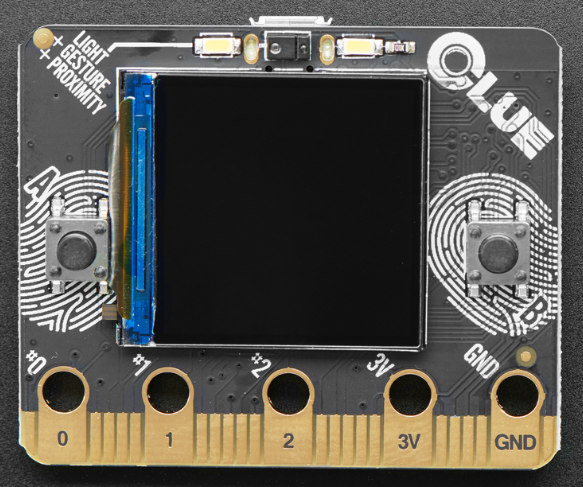
\includegraphics[scale=0.4]{Report/Images/ClueBoard.png}
    \caption{Adafruit CLUE board \cite{learnAdafruit}}
    \label{fig:adafruitClue}
\end{figure}

\subsection{CircuitPython}

CircuitPython is a programming language designed to be easy for beginners and experienced programmers alike to develop their own interactive projects. It adds hardware support to Python with libraries that allow you to code on low-cost microcontrollers and single board computers \cite{circuitpython}.

As Adafruit also supports the development of CircuitPython, it was the ideal programming language to code the experiments with. The boards using CircuitPython provide quick feedback which allow the programming of the experiments and libraries to be simple yet flexible.

\subsection{Kitronik Smart Greenhouse}

To run the experiments, the Kitronik Smart Greenhouse kit for BBC Micro:bit will be used. The CLUE board already has temperature and humidity sensors built in, alongside a handful of other useful components. The greenhouse kit provides an additional moisture sensor which can be connected to the board using crocodile clips, which are also provided. This will sit in the soil to regularly monitor the moisture levels. A motor and zip LEDs are also provided to allow control over how frequently the plant is watered and the level of light the plant is exposed to.

\begin{figure}[ht]
    \centering
    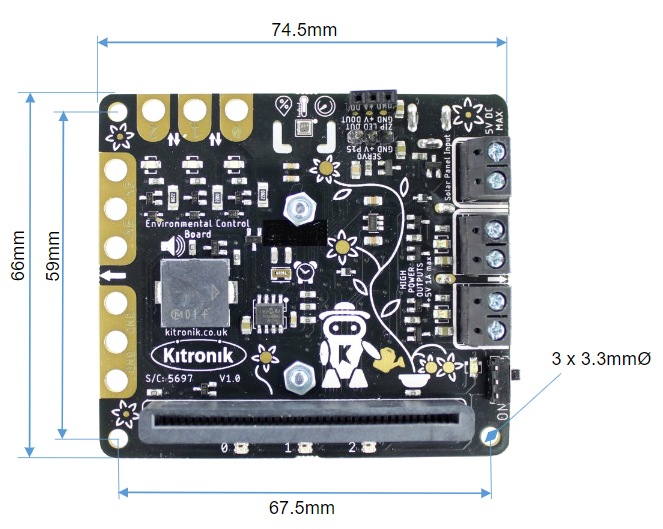
\includegraphics[scale=0.6]{Report/Images/KitronikBoard.png}
    \caption{Kitronik Environmental Control Board \cite{kitronikBoard}}
    \label{fig:KitronikBoard}
\end{figure}

\begin{figure}[ht]
    \centering
    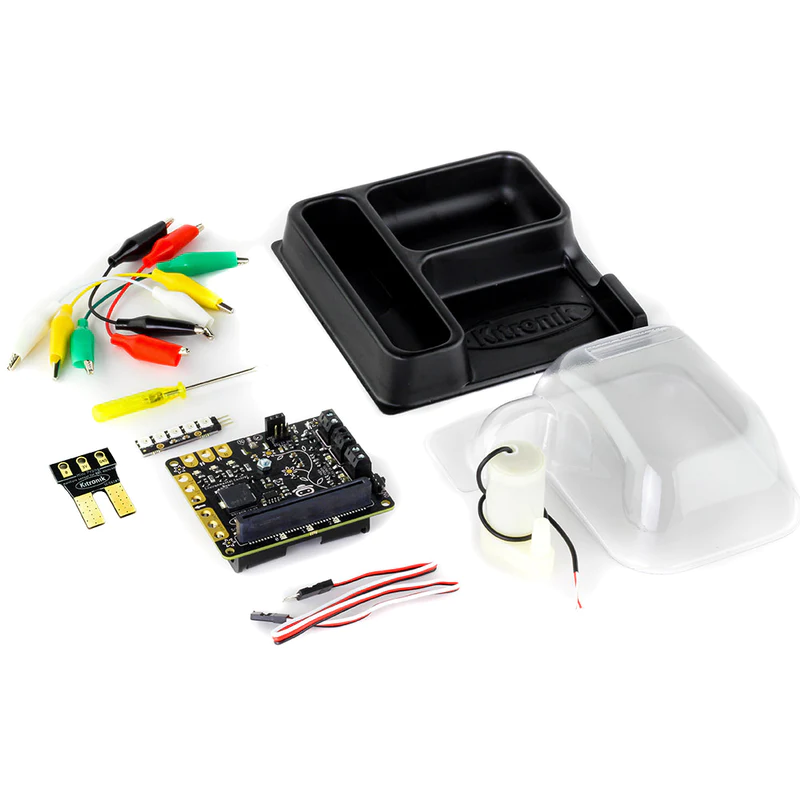
\includegraphics[scale=0.4]{Report/Images/KitronikGreenhouse.png}
    \caption{Kitronik Smart Greenhouse \cite{kitronikStore}}
    \label{fig:KitronikGreenhouse}
\end{figure}
